\documentclass{beamer}
\usetheme{Madrid}


\usepackage{graphicx}
\usepackage{xcolor}


\definecolor{myred}{RGB}{255,0,0}
\setbeamercolor{structure}{fg=myred}
\setbeamercolor{block title}{bg=myred,fg=white}


\title{NRO DN 1}
\author{Adam Valjavec}
\institute{Fakulteta za strojništvo}
\date{\today}

\begin{document}

\begin{frame}
  \titlepage

  \begin{figure}
    
\includegraphics[width=0.3\linewidth]{ul-fakulteta-za-strojnistvo.jpg}
   
  \end{figure}
\end{frame}

\begin{frame}{Kazalo}
  \tableofcontents
\end{frame}

\section{Metoda Monte Carlo}
\begin{frame}{Metoda Monte Carlo}
  Z metodo Monte Carlo smo s pomočjo Matlab-a izračunali približek števila pi.
  

  \begin{figure}
    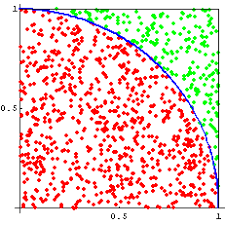
\includegraphics[width=0.3\linewidth]{monte_carlo_and_pi_zv.png}
    \caption{Grafični prikaz metode Monte Carlo}
  \end{figure}
\end{frame}

\section{GitHub}
\begin{frame}{GitHub}
  Našo domačo nalogo smo:
  \begin{itemize}
    \item Naložili na GitHub \pause
    \item Pomagali kolegu in mu dodali oznake na oseh, naslov...
  \end{itemize}
\end{frame}

\section{Beamer}
\begin{frame}{Beamer}
 V Overleafu smo naredili predstavitev DN.
  
\end{frame}



\end{document}